\chapter{Aufbau}
\label{ch:Aufbau}
Dieses Kapitel beschreibt den konkreten Aufbau der Testbench. Wie in Sektion \ref{sec:Architektur und Technologien:Architektur} beschrieben, ist die verwendete Architektur Event-basiert. Abbildung \ref{fig:classDiagram} skizziert eine vereinfachte Form der Testbench in einer UML-Klassendiagramm ähnlichen Form. Aus Übersichtsgründen sind Utility-Klassen, Transfer-Objekte, POJO's\footnote{Plain Old Java Objects: Werden bspw. für die JSON-Deserialisierung benutzt} und die Event-Listener und Event-Publisher der Komponenten nicht Teil des Diagramms. 





%"l, b, r, t"
\begin{figure}[t]
	\centering
	\begin{sideways}
		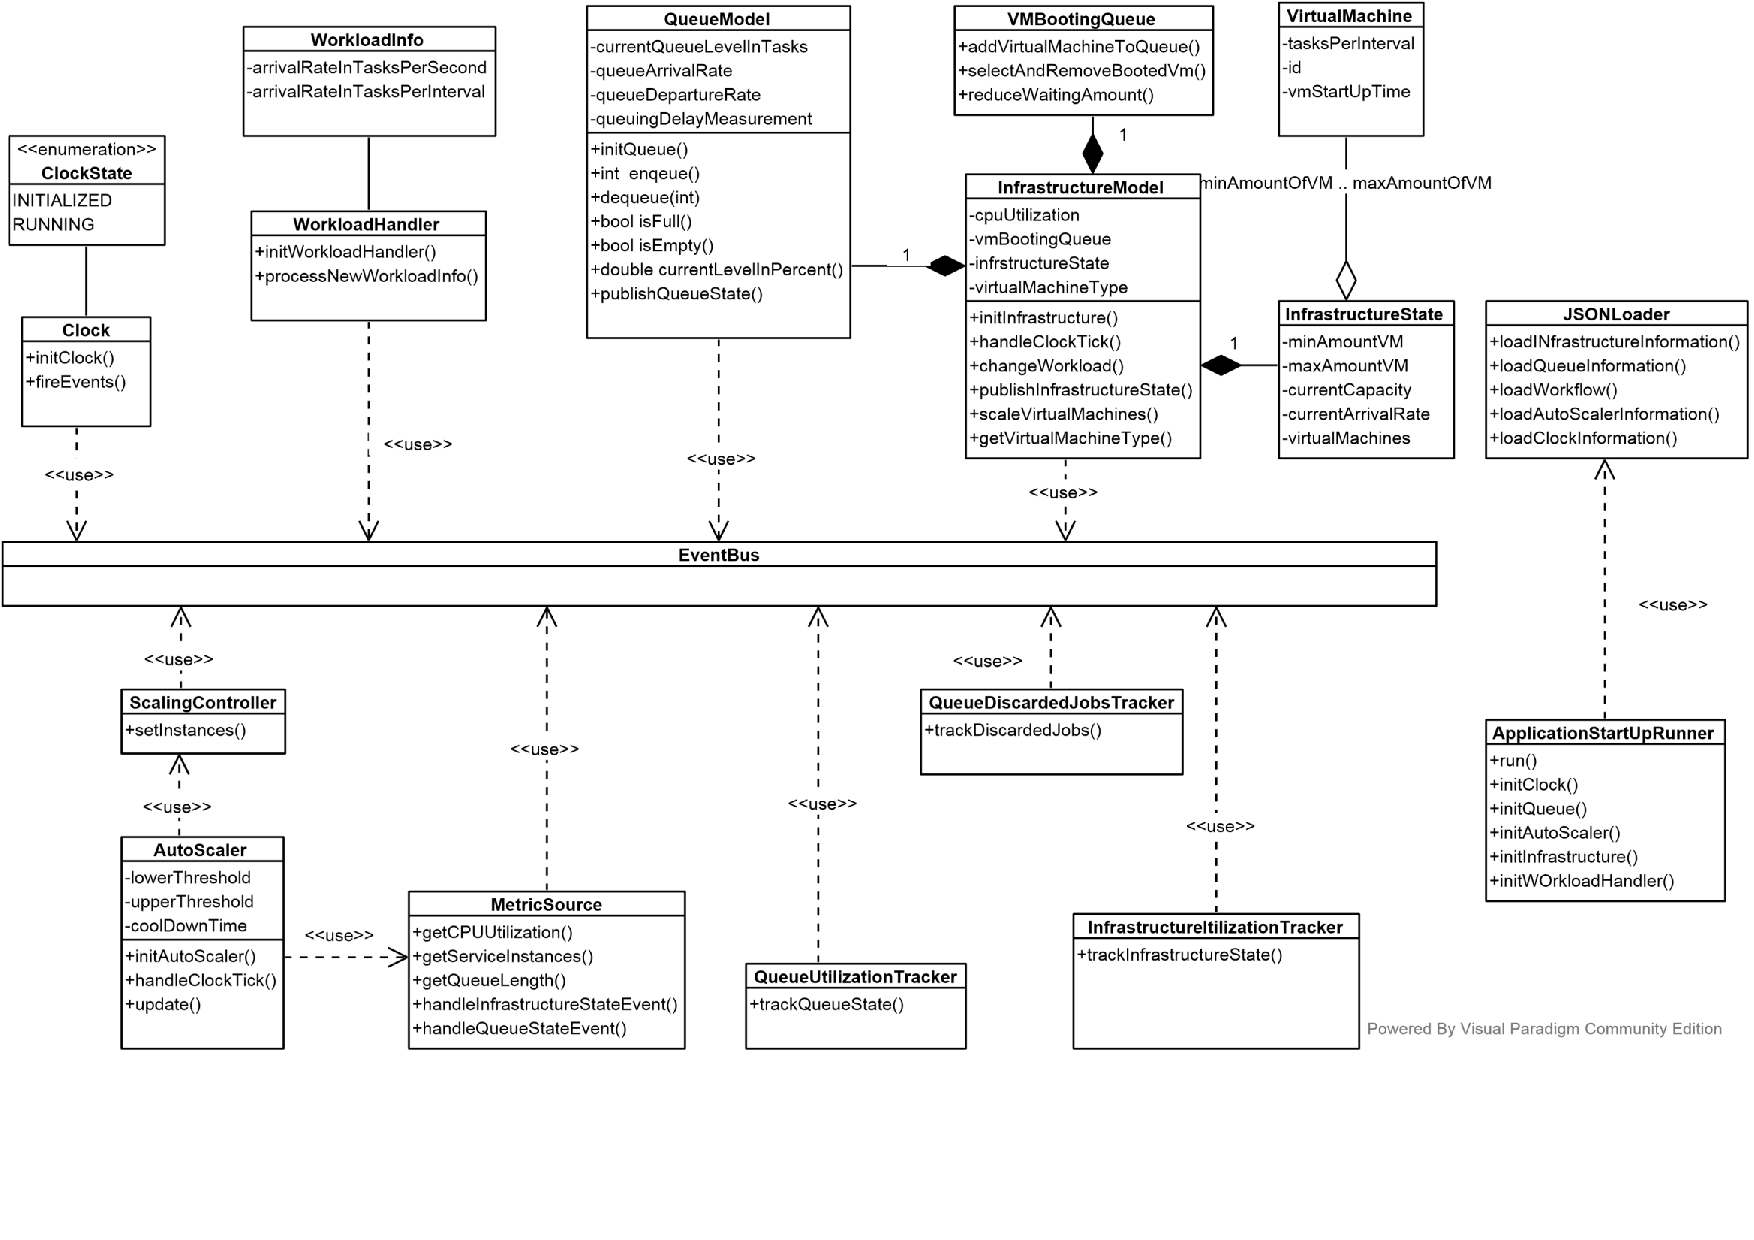
\includegraphics[width=20.0cm, trim={0cm 0cm 0cm 0cm}]{img/classDiagram.pdf}
	\end{sideways}
		\caption{Aufbau des Auto-Skalierers}
	\label{fig:classDiagram}
\end{figure}


\section{Komponenten}
test

\subsection{Clock}
test

\subsection{Infrastructure Model}

\subsubsection{VM Booting Queue}

\subsection{Infrastructure State}

\subsection{Virtual Machine}


\subsection{Auto Scaler}

\subsubsection{Scaling Controller}

\subsubsection{Metric Source}




\subsection{Queue Model}


\subsection{Workload Handler}

\subsubsection{Workload Info}


\subsection{Tracker}

\subsubsection{Queue Utilization Tracker}

\subsubsection{Queue Discarded Jobs Tracker}

\subsubsection{Infrastructure Utilization Tracker}

\subsection{Application Start Up Runner}

\subsection{JSON Loader}

\section{Events}

